\documentclass[
  bibliography=totoc,     % Literatur im Inhaltsverzeichnis
  captions=tableheading,  % Tabellenüberschriften
  titlepage=firstiscover, % Titelseite ist Deckblatt
]{scrartcl}

% Paket float verbessern
\usepackage{scrhack}

% Warnung, falls nochmal kompiliert werden muss
\usepackage[aux]{rerunfilecheck}

% unverzichtbare Mathe-Befehle
\usepackage{amsmath}
% viele Mathe-Symbole
\usepackage{amssymb}
% Erweiterungen für amsmath
\usepackage{mathtools}

% Fonteinstellungen
\usepackage{fontspec}
% Latin Modern Fonts werden automatisch geladen
% Alternativ:
%\setromanfont{Libertinus Serif}
%\setsansfont{Libertinus Sans}
%\setmonofont{Libertinus Mono}
\recalctypearea % Wenn man andere Schriftarten gesetzt hat,
% sollte man das Seiten-Layout neu berechnen lassen

% deutsche Spracheinstellungen
\usepackage{polyglossia}
\setmainlanguage{german}


\usepackage[
  math-style=ISO,    % ┐
  bold-style=ISO,    % │
  sans-style=italic, % │ ISO-Standard folgen
  nabla=upright,     % │
  partial=upright,   % ┘
  warnings-off={           % ┐
    mathtools-colon,       % │ unnötige Warnungen ausschalten
    mathtools-overbracket, % │
},                       % ┘
]{unicode-math}

% traditionelle Fonts für Mathematik
\setmathfont{Latin Modern Math}
% Alternativ:
%\setmathfont{Libertinus Math}

\setmathfont{XITS Math}[range={scr, bfscr}]
\setmathfont{XITS Math}[range={cal, bfcal}, StylisticSet=1]

% Zahlen und Einheiten
\usepackage[
locale=DE,                   % deutsche Einstellungen
separate-uncertainty=true,   % immer Fehler mit \pm
per-mode=symbol-or-fraction, % / in inline math, fraction in display math
alsoload=<torr>
]{siunitx}

% chemische Formeln
\usepackage[
version=4,
math-greek=default, % ┐ mit unicode-math zusammenarbeiten
text-greek=default, % ┘
]{mhchem}

% richtige Anführungszeichen
\usepackage[autostyle]{csquotes}

% schöne Brüche im Text
\usepackage{xfrac}

% Standardplatzierung für Floats einstellen
\usepackage{float}
\floatplacement{figure}{htbp}
\floatplacement{table}{htbp}

% Floats innerhalb einer Section halten
\usepackage[
section, % Floats innerhalb der Section halten
below,   % unterhalb der Section aber auf der selben Seite ist ok
]{placeins}

% Seite drehen für breite Tabellen: landscape Umgebung
\usepackage{pdflscape}

% Captions schöner machen.
\usepackage[
  labelfont=bf,        % Tabelle x: Abbildung y: ist jetzt fett
  font=small,          % Schrift etwas kleiner als Dokument
  width=0.9\textwidth, % maximale Breite einer Caption schmaler
]{caption}
% subfigure, subtable, subref
\usepackage{subcaption}

% Grafiken können eingebunden werden
\usepackage{graphicx}
% größere Variation von Dateinamen möglich
\usepackage{grffile}

% schöne Tabellen
\usepackage{booktabs}

% Verbesserungen am Schriftbild
\usepackage{microtype}

% Literaturverzeichnis
\usepackage[style=alphabetic,]{biblatex}
% Quellendatenbank
\addbibresource{lit.bib}

% Hyperlinks im Dokument
\usepackage[
  unicode,        % Unicode in PDF-Attributen erlauben
  pdfusetitle,    % Titel, Autoren und Datum als PDF-Attribute
  pdfcreator={},  % ┐ PDF-Attribute säubern
  pdfproducer={}, % ┘
]{hyperref}
% erweiterte Bookmarks im PDF
\usepackage{bookmark}

% Trennung von Wörtern mit Strichen
\usepackage[shortcuts]{extdash}

\title{V503: Der Millikan-Öltröpfchenversuch}
\author{
  Simon Schulte
  \texorpdfstring{
    \\
    \href{mailto:simon.schulte@udo.edu}{simon.schulte@udo.edu}
  }{}
  \texorpdfstring{\and}{, }
  Tim Sedlaczek
  \texorpdfstring{
    \\
    \href{mailto:tim.sedlaczek@udo.edu}{tim.sedlaczek@udo.edu}
  }{}
}
\publishers{TU Dortmund – Fakultät Physik}

\date{Durchführung: 16.05.2017\\
      Abgabe: 23.05.2017}


\begin{document}

\maketitle
\thispagestyle{empty}
\tableofcontents
\newpage
\setcounter{page}{1}
\section{Zielsetzung}
\label{sec:zielsetzung}
Bei dem Millikan-Öltröpfchenversuch wir anhand der Bewegungen
eines geladenen Öltröpfchens im Feld eines Plattenkondensators.
Die Elementarladung bestimmt.

\noindent
Bei dem regulären Verfahren wird dazu die Geschwindigkeit des Tröpfchens,
für einen abgeschalteten Kondensator und für die zwei verschiedenen
Möglichkeiten der Polarisierung des Kondensators, bei bekannten Spannungen
gemessen.
Hier wird jedoch ein leicht verändertes Verfahren verwendet.
\section{Theorie}
\label{sec:theorie}
Beim einsprühen des Öls in die Apparatur werden die Öltröpfchen
durch Reibung geladen. Zwischen den Kondensatorplatten
erfahren sie dann mehrere Kräfte:

\noindent
Die Gewichtskraft
\begin{equation}
  \vec{F}_ \mathup{g} = m \cdot \vec{g},
\end{equation}
die Stokesche Reibung
\begin{equation}
  \vec{F}_\mathup{R} = - 6 \pi r \eta_\mathup{L} \vec{v}
\end{equation}
und, bei eingeschaltetem Kondensator, die elektrische Kraft
\begin{equation}
  \vec{F}_\mathup{el} = q \cdot \vec{E}.
\end{equation}
$g$ ist dabei die Schwerebeschleunigung, $r$ der Radius des Tröpfchens, $\eta_\mathup{L}$
die Viskosität der Luft und $E$ die elektrische Feldstärke im Kondensator.

\noindent
Bei einem Kräftegleichgewicht bewegen sich die Tröpfchen mit konstanter
Geschwindigkeit $v$.
Zunächst wird das Gleichgewicht bei abgeschaltetem Kondensator betrachtet.
Dabei sind die Gewichtskraft und die Stokesche Reibung betragsweise gleich
groß. Durch umschreiben der Masse $m$ in ein Produkt aus Dichte $\rho$ und
Volumen $\frac{4 \pi}{3}r^3$ folgt:
\begin{equation}
  \frac{4 \pi}{3}r^3 \rho g = 6 \pi \eta_\mathup{L} r v_0.
  \label{eqn:kräftegleichgew}
\end{equation}
Daraus folgt der Tröpfchenradius
\begin{equation}
  r = \sqrt{\frac{9 \eta_\mathup{L} v_0}{2 g \rho}}.
  \label{eqn:tröpfchenradius}
\end{equation}
Zur Bestimmung der Ladung wird der Kondensator eingeschaltet und eine ausreichend
große Spannung angelegt, sodass das Tröpfchen in der Luft schwebt. In diesem Fall
sind die elektrische Kraft und die Gewichtskraft im Gleichgewicht:
\begin{equation}
  \frac{4 \pi}{3}r^3 \rho g = q \cdot E = q \cdot \frac{U}{d}
  \label{eqn:gleichgewicht}
\end{equation}
Daraus folgt die Ladung des Tröpfchens
\begin{equation}
  q = \frac{4 \pi}{3}r^3 \rho g \frac{d}{U}
  \label{eqn:ladung}
\end{equation}

\noindent
Da die Stokesche Reibung so wie sie bisher verwendet wurde nur für Tröpfchen gilt,
die größer sind als die mittlere freie Weglänge in Luft, muss die Viskosität
der Luft korrigiert werden:
\begin{equation}
  \eta_{eff} = \eta_\mathup{L} \Biggl( \frac{1}{1+\frac{B}{pr}} \Biggr).
  \label{eqn:korrvisk}
\end{equation}
Hierbei ist $B = \SI{6.17e-3}{\torr\centi\meter}$ und $p$ der Luftdruck.
Daraus ergibt sich die korrigierte Ladung
\begin{equation}
  q_\mathup{Korr} = q_0 \biggl( 1 + \frac{B}{pr} \biggr)^{-\frac{3}{2}}.
  \label{eqn:korrlad}
\end{equation}
\section{Durchführung}
\label{sec:durchführung}
\subsection{Versuchsaufbau}
\begin{figure}[htb]
  \centering
  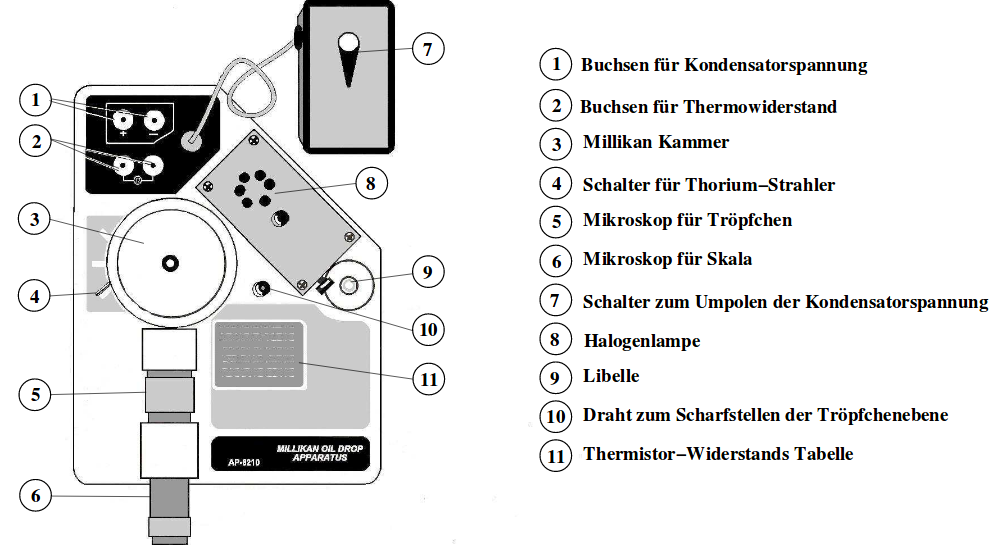
\includegraphics[width=0.9\textwidth]{5031.png}
  \caption{Der Versuchsaufbau. \cite{anleitung}}
  \label{fig:5031}
\end{figure}
In Abbildung \ref{fig:5031} ist der Aufbau der Apparatur für den Millikanversuch
dargestellt.

\noindent
An den Buchsen 1 und 2 kann die tatsächlich am Kondensator anliegende Spannung
und der thermische/elektrische Widerstand der Luft gemessen werden.
Über den Widerstand wird dann während des Versuchs die Temperatur im Innern des
Kondensators bestimmt. Für den Fall, dass die Öltröpfchen nicht hinreichend geladen sein sollten,
ist ein Alphastrahler in die Apparatur integriert. Dieser ist von der Kammer abgeschirmt.
Um dir Abschirmung kurzzeitig zu entfernen kann der Hebel 4 in die "On" Stellung
gelegt werden. Mit dem Mikroskop wird das Innere der Kammer aufgenommen und auf
einem Bildschirm angezeigt. Das Bild kann an dem Mikroskop auf die Tröpfchenebene
und auf die Skala fokussiert werden. Damit die Tröpfchen nicht seitlich abdriften
muss die Apparatur möglichst gerade ausgerichtet sein. Die Libelle 9 zeigt dabei
die Neigung an.
\subsection{Versuchsablauf}
Zu Beginn der Messung wird an der Oberseite, der Millikan Kammer, Öl zerstäubt.
An dem Bildschirm können dann die Tröpfchen beobachtet werden.

\noindent
Führ die Messung wird ein relativ langsames Tröpfchen gewählt.
Durch einschalten des Kondensators wird geprüft ob das Tröpfchen
geladen ist. Wenn sich ein Tröpfchen entsprechend für die Messung
eignet wird die Zeit gestoppt, die es bei abgeschaltetem Kondensator
benötigt, um $\SI{0.5}{\milli\meter}$ zurückzulegen. Anschließend wird
mit dem Generator eine Spannung eingestellt, die so groß ist, dass das
Tröpfchen in der Luft ruht. Die eingestellte Spannung wird dann zusammen
mit der aktuellen Temperatur in der Kammer notiert.

\noindent
Wenn keine passenden Tröpfchen auf dem Bild zu sehen sind kann durch
Pusten dafür gesorgt werden, dass neue Öltröpfchen vor das Mikroskop
gelangen. Sollte dies nicht weiter helfen wird neues Öl in der Kammer
zerstäubt. Die Messung der Fallzeit, der Spannung und der Temperatur
wird für $25$ Tröpfchen durchgeführt.
\clearpage

%Hier ist Platz für die Auswertung ;)

\nocite{*}
\printbibliography
\end{document}
